\documentclass[xcolor=svgnames]{beamer}
\mode<presentation>
{
      \setbeamertemplate{footline}[page number]
      \setbeamercovered{transparent}
      \setbeamertemplate{navigation symbols}{}
      \usecolortheme[named=DarkGreen]{structure}
}

\usepackage[english]{babel}
\usepackage{times}
\usepackage{url}
\usepackage{CJKutf8}
\usepackage{graphics}

\begin{document}
\begin{CJK*}{UTF8}{gbsn}


\title{操作系统概论}

\author{李中国}
\institute{苏州大学计算机科学与技术学院}
%\date{2011年5月30日}
\date{}

\begin{frame}
  \titlepage
\end{frame}


\begin{frame}{虚拟机软件及Ubuntu操作系统下载地址}
\begin{description}
\item[虚拟机软件VirtualBox:] \url{www.virtualbox.org}
\item[Ubuntu操作系统:] \url{www.ubuntu.com}
\end{description}
\end{frame}

\begin{frame}{安装Ubuntu 11.10操作系统: ISO文件}
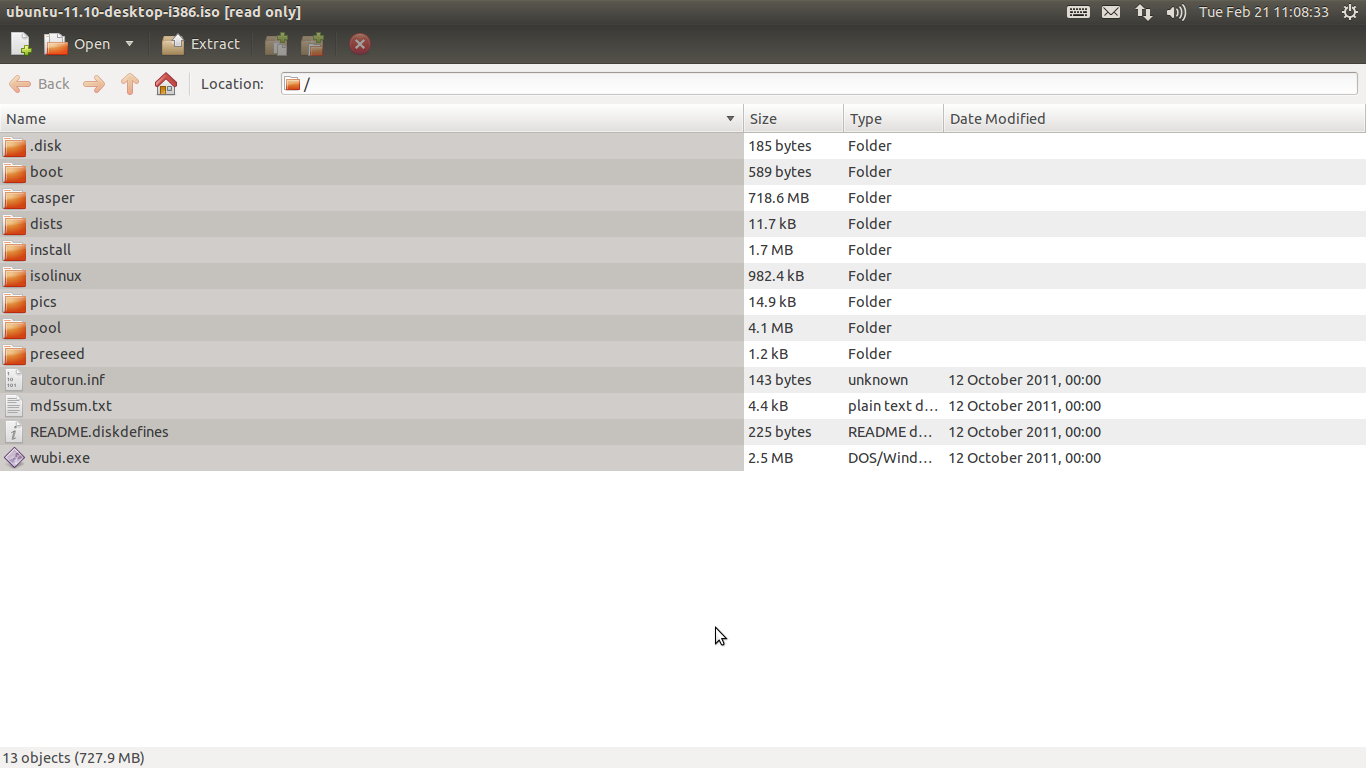
\includegraphics[width=1.5\textwidth]{ubuntu-iso.png}
\end{frame}

\begin{frame}{用Wubi安装Ubuntu 11.10操作系统}
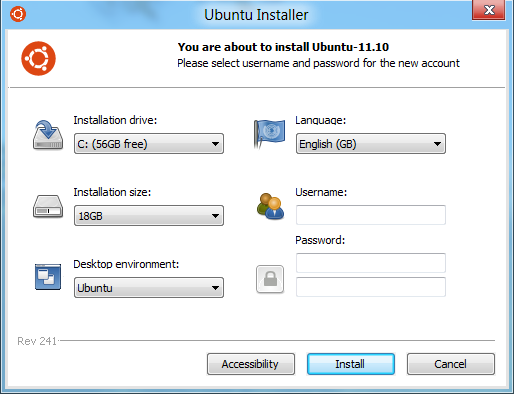
\includegraphics[width=0.9\textwidth]{wubi.png}
\end{frame}

\begin{frame}{用Wubi安装Ubuntu以后的启动界面}
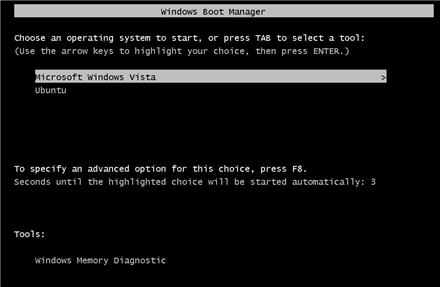
\includegraphics[width=0.9\textwidth]{boot-screen.jpg}
\end{frame}

\begin{frame}{Ubuntu 11.10图形界面}
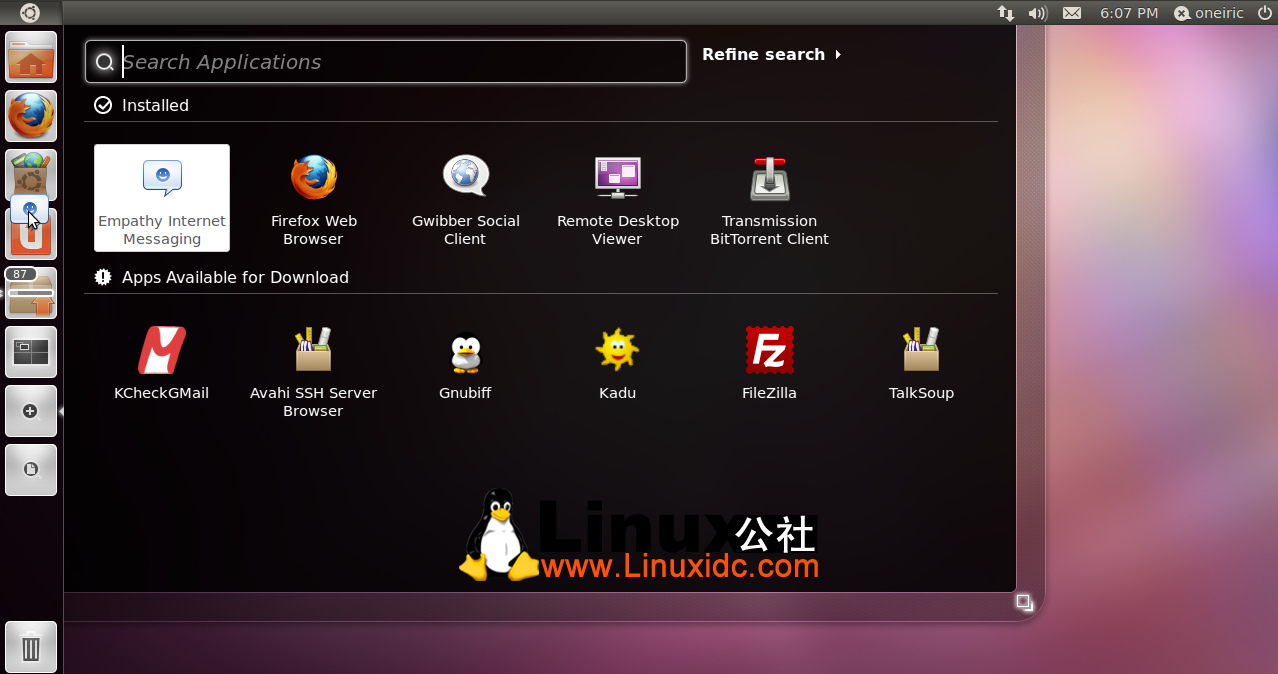
\includegraphics[width=1.0\textwidth]{ubuntu-1110.jpg}
\end{frame}

\begin{frame}{卸载Wubi安装的Ubuntu 11.10}
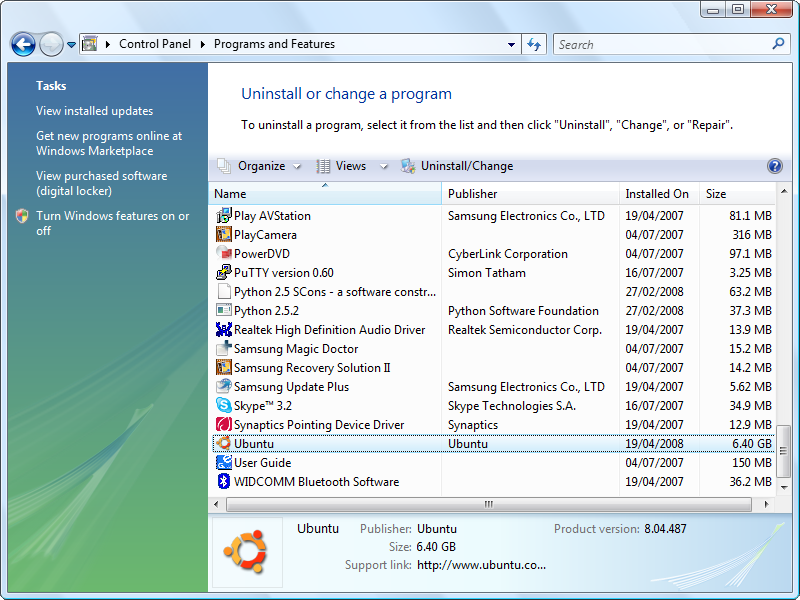
\includegraphics[width=0.9\textwidth]{uninstall.png}
\end{frame}

\begin{frame}{课程内容}
\begin{itemize}
\item 操作系统概念及理论
\item 阅读操作系统源代码并完成编程作业
\item 学习本课程的知识要求:
\begin{itemize}
\item C语言程序设计
\item 数据结构
\item 计算机组成原理
\item 计算机体系结构
\item 汇编语言程序设计
\end{itemize}
\end{itemize}
\end{frame}

\begin{frame}{课程要求及考核方法}
\begin{itemize}
\item 期末考试: 50\%
\item 平时作业(程序设计): 50\%
\item 两项均需及格方能通过本课程
\begin{description}
\item[Pass:] 30, 30
\item[Fail:] 50, 10
\item[Excellent:] 40+, 40+
\end{description}
\item 两点要求:
\begin{description}
\item[编程作业] 需要独立完成
\item[课堂考勤]要求 
\end{description}
\end{itemize}
\end{frame}

\begin{frame}{什么是操作系统}
\begin{columns}%[t]
\column{.5\textwidth}
\begin{itemize}
\item 介于\alert{用户}与计算机硬件之间的程序 
\item 思考: 操作系统的用户
\item 操作系统的设计目标
\begin{itemize}
\item 执行用户程序
\item 使计算机系统易于使用
\item 高效利用计算机硬件
\end{itemize}
\item 对比:应用软件的设计目标
\end{itemize}
\column{.5\textwidth}

\includegraphics[width=.9\textwidth]{frustrated-user.jpeg}
\end{columns}
\end{frame}

\begin{frame}{为什么学习操作系统}
\begin{itemize}
\item 计算机系统的不可缺少的关键部分
\item 非常复杂 
\begin{itemize}
\item Linux Kernel 2.6.35 --- 13.5 M
\item FreeBSD --- 8.8 M 
\item Mac OS X 10.4 --- 86 M 
\item Windows Server 2003 -- 50 M
\end{itemize}
\item 真正理解计算机系统的工作原理
\item 涉及硬件、编程语言、数据结构、算法等多个领域
\end{itemize}
\end{frame}

\begin{frame}{计算机系统组成}
\begin{itemize}
\item 计算机硬件: 提供基本计算资源
\begin{itemize}
\item CPU, Memory, I/O devices...
\end{itemize}
\item 操作系统
\begin{itemize}
\item 控制、协调用户和程序对硬件资源的使用
\end{itemize}
\item 应用程序: 解决用户的计算问题
\begin{itemize}
\item Word processors, compilers, web browsers, database
systems, video games
\end{itemize}
\item 用户
\begin{itemize}
\item People, machines (other computers)
\end{itemize}
\end{itemize}
\end{frame}

\begin{frame}{计算机系统组成}
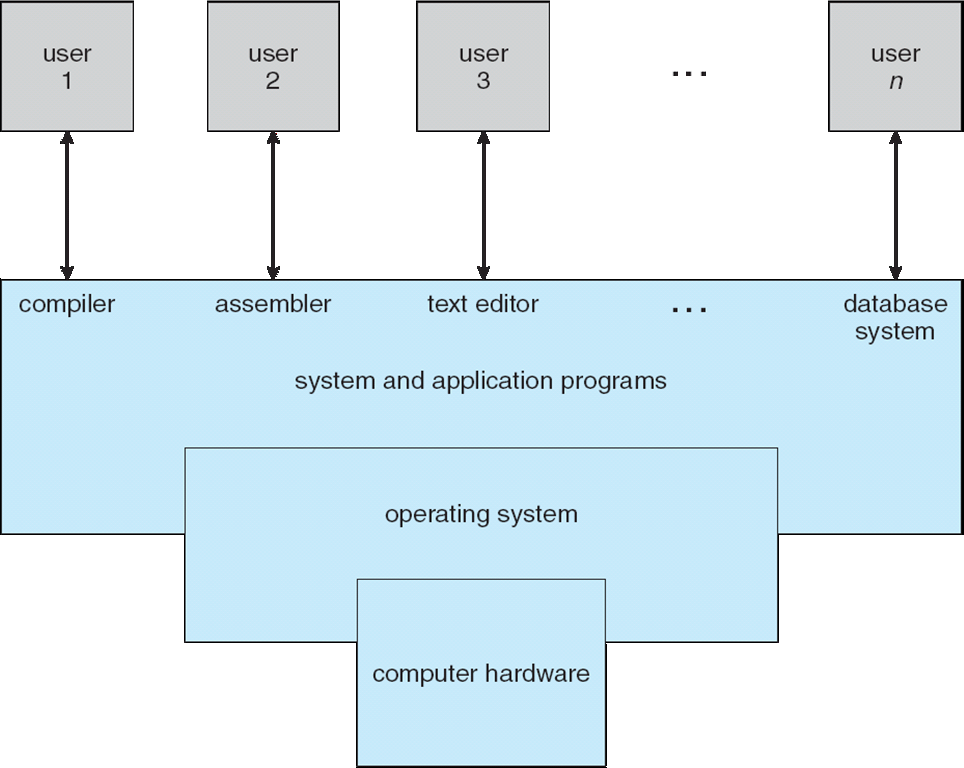
\includegraphics[width=.9\textwidth]{system.png}
\end{frame}

\begin{frame}{操作系统的作用}
\begin{itemize}
\item 提供容易使用的界面(终端用户及程序员)
\item 最大限度地提高资源利用率(CPU,内存)
\item 为多用户提供分时服务(time sharing system)
\item 在多用户多系统之间实现资源共享(存储、打印机)
\item 嵌入式设备:界面问题、电池寿命问题(不只是OS的任务)
\end{itemize}
\end{frame}

\begin{frame}{操作系统的作用: 资源管理}
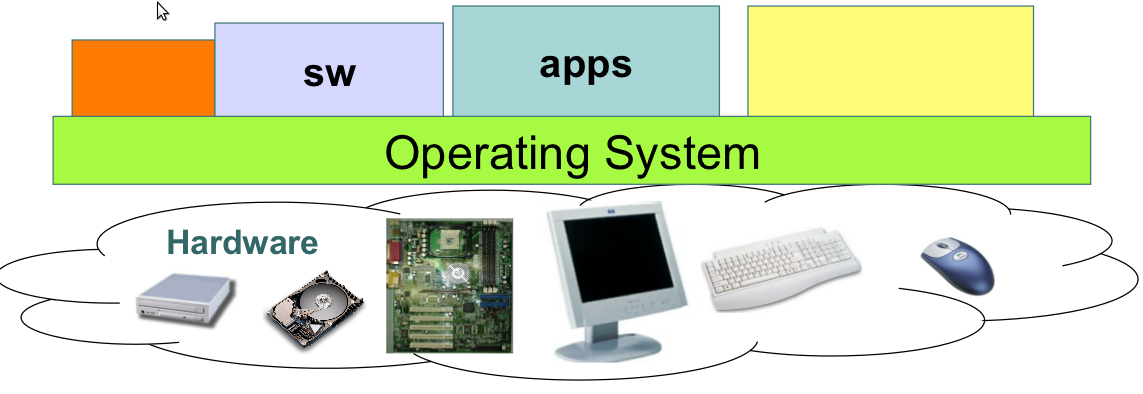
\includegraphics[width=1.0\textwidth]{os-function.png}
\end{frame}

\begin{frame}{操作系统的作用: 提供易于使用的界面}
%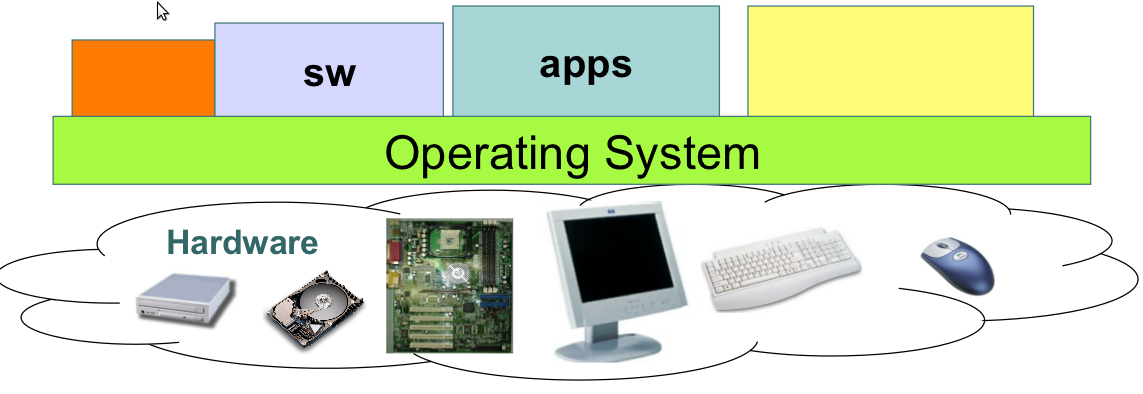
\includegraphics[width=1.0\textwidth]{os-function.png}
\begin{columns}
\column{.5\textwidth}
\column{.5\textwidth}
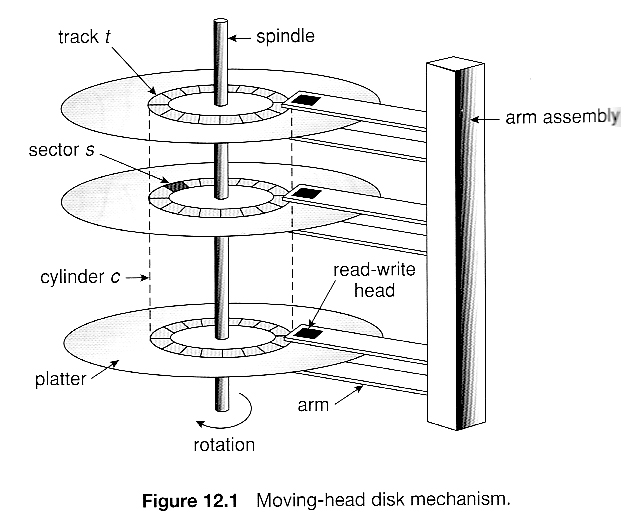
\includegraphics[width=1.0\textwidth]{disk.jpg}
\end{columns}
\end{frame}

\begin{frame}{计算机硬件系统}
\begin{itemize}
\item CPUs, 设备控制器等通过总线与内存连接
\item 竞争内存周期, 实现CPU、设备控制器间的并发执行
\end{itemize}
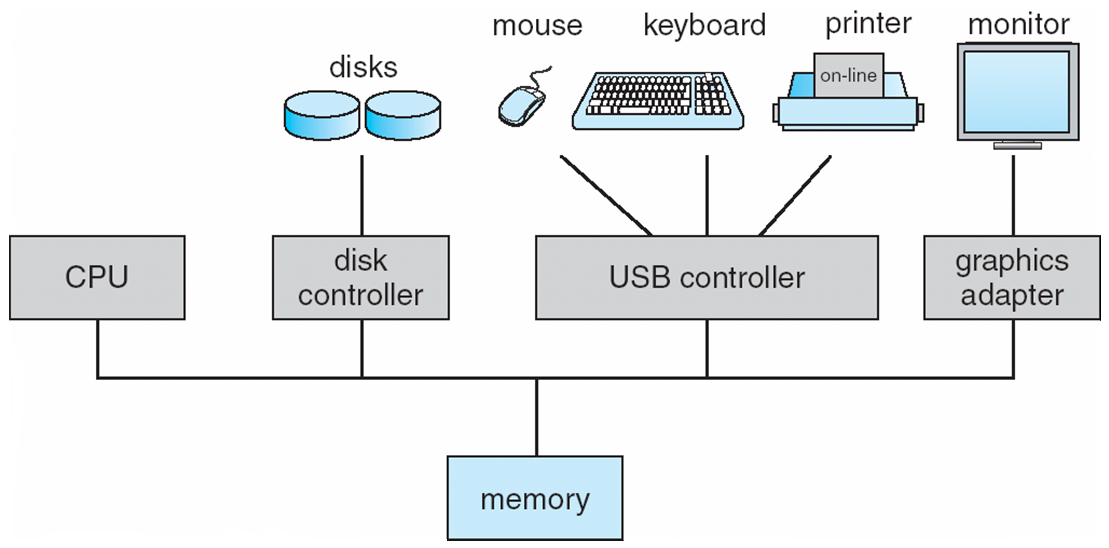
\includegraphics[width=1.0\textwidth]{org.png}
\end{frame}

\begin{frame}{计算机硬件系统}
\begin{itemize}
\item I/O设备与CPU可以并发运行
\item 每个设备控制器控制一种I/O设备
\item 设备控制器有自己的本地缓存
\item CPU --- 内存 --- 设备缓存 --- 设备
\item I/O: 从设备到设备控制器的缓存
\item I/O完成后,设备控制器通过\alert{中断}通知OS
\end{itemize}
\end{frame}

\begin{frame}{中断(interrupt)}
\begin{itemize}
\item 操作系统由中断驱动
\item 硬件中断与软件中断
\end{itemize}
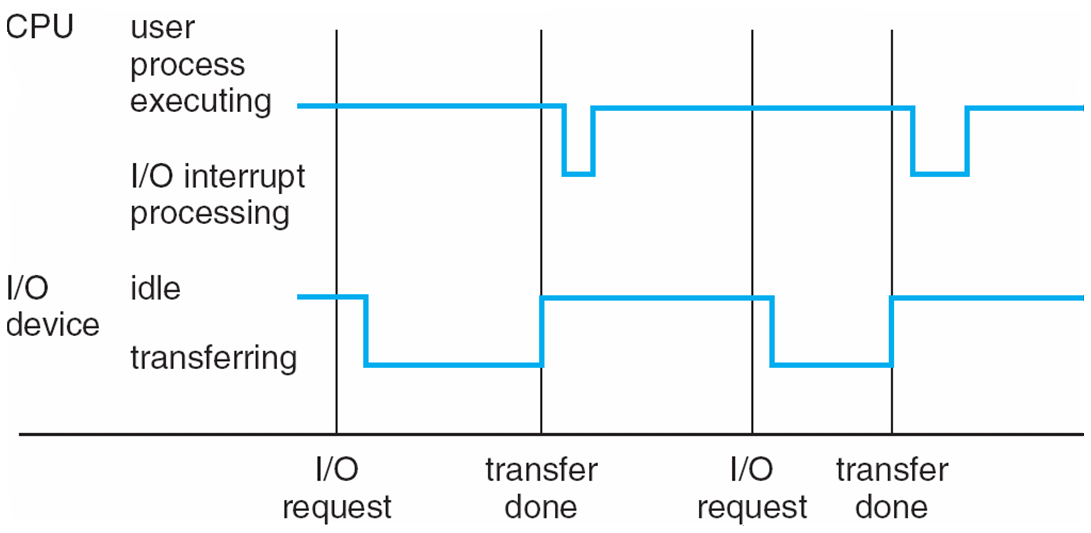
\includegraphics[width=1.0\textwidth]{interrupt.png}
\end{frame}

\begin{frame}{直接内存访问(DMA)}
\begin{itemize}
\item 高速I/O设备与内存之间采用DMA传输数据
\item 每传输1块数据产生一个中断
\end{itemize}
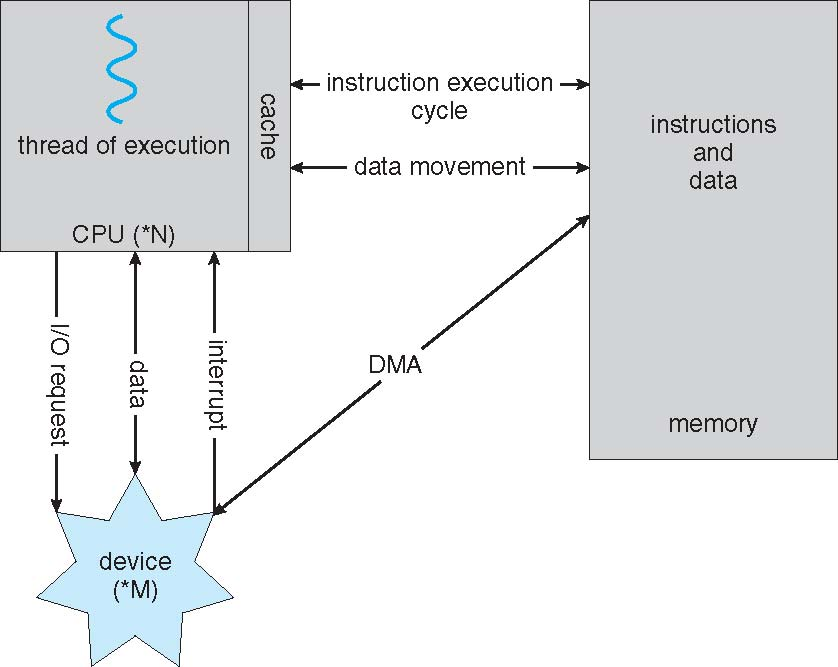
\includegraphics[width=0.8\textwidth]{vonneumann.jpg}
\end{frame}

\begin{frame}{存储层级}
\begin{columns}
\column{.3\textwidth}
\begin{itemize}
\item 存取速度
\item 制造成本
\item Caching技术
\end{itemize}
\column{.7\textwidth}
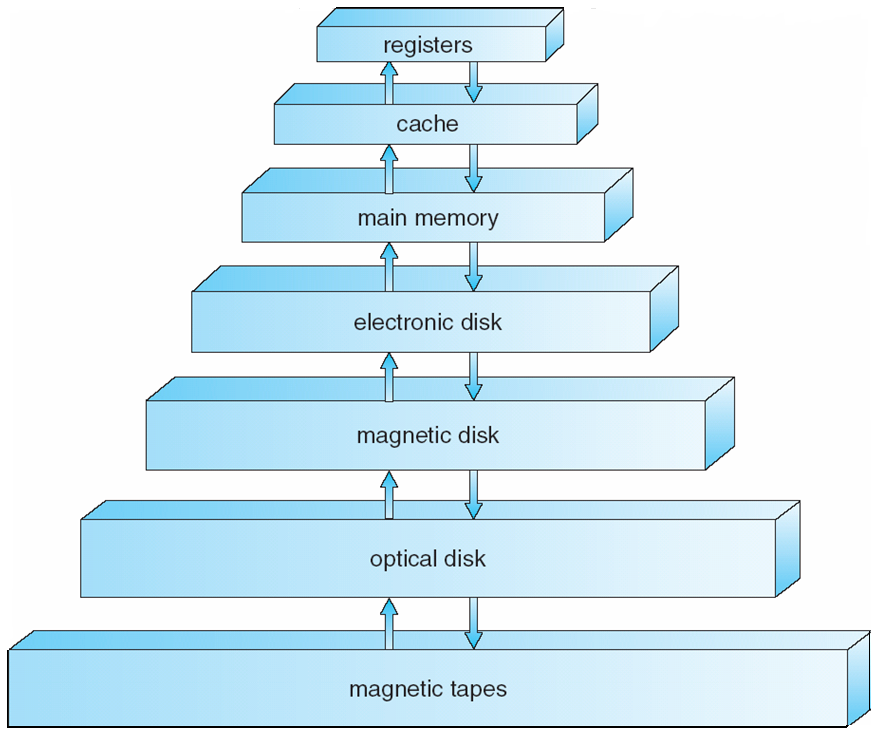
\includegraphics[width=0.9\textwidth]{storage.png}
\end{columns}
\end{frame}

\begin{frame}{多道程序设计与分时系统}
\begin{columns}
\column{.3\textwidth}
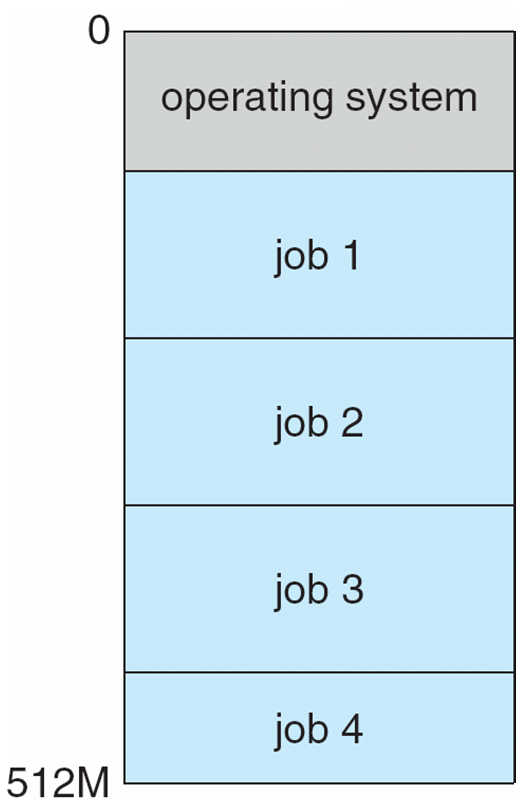
\includegraphics[width=1.0\textwidth]{jobs.png}
\column{.7\textwidth}
\begin{itemize}
\item 多道程序设计(multiprogramming)
\begin{itemize}
\item 单个用户或程序无法使CPU或外设保持忙碌 
\item 引入多道程序设计技术
\item 多个作业(jobs)驻留内存
\item 操作系统需要进行作业调度
\item 需要等待I/O时,调入另一作业运行
\end{itemize}
\item 分时系统(timesharing system)与交互式计算(interactive computing)
\end{itemize}
\end{columns}
\end{frame}

\begin{frame}{核心态与用户态}
\begin{itemize}
\item 核心态: 执行操作系统代码
\item 用户态: 执行用户程序代码
\item 思考:哪些指令需要在核心态下执行?
\item 系统调用导致从用户态转入核心态
\end{itemize}
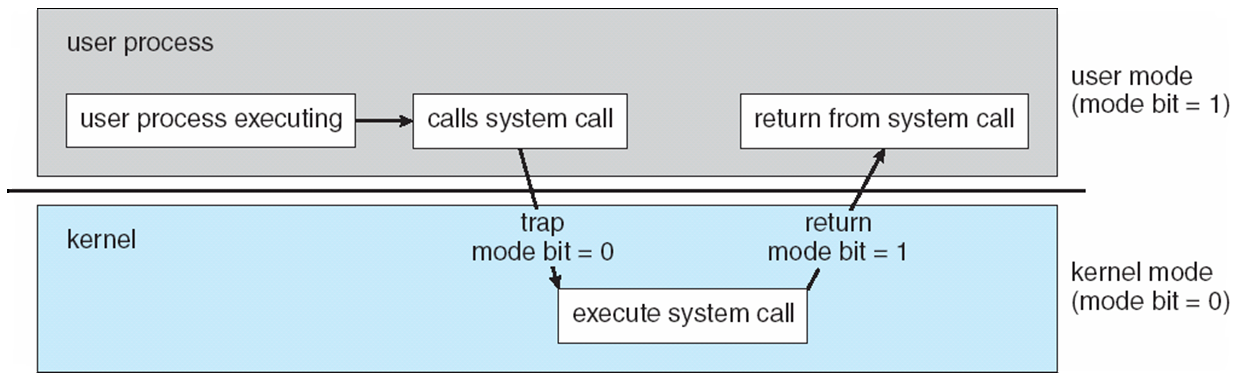
\includegraphics[width=1.0\textwidth]{mode.png}
\end{frame}

%\begin{frame}{进程管理}
%\begin{itemize}
%\item 
%\end{itemize}
%\end{frame}

\end{CJK*}
\end{document}
